\documentclass[10pt]{article}
\usepackage[polish]{babel}
\usepackage[utf8]{inputenc}
\usepackage[T1]{fontenc}
\usepackage{amsmath}
\usepackage{amsfonts}
\usepackage{amssymb}
\usepackage[version=4]{mhchem}
\usepackage{stmaryrd}
\usepackage{graphicx}
\usepackage[export]{adjustbox}
\graphicspath{ {./images/} }

\title{LIGA MATEMATYCZNA \\
 im. Zdzisława Matuskiego LISTOPAD 2017 \\
 SZKOŁA PODSTAWOWA }

\author{}
\date{}


\begin{document}
\maketitle
\section*{ZADANIE 1.}
Mikołaj zrobił sok malinowy na zimę i wlał go do trzylitrowych butelek. Potem jednak postanowił przelać sok do pięciolitrowych słojów. Okazało się, że jedenaście słojów to za mało, więc wlał sok po równo do dwunastu takich słojów, chociaż teraz nie są one pełne. Ile soku jest w każdym słoju?

\section*{ZADANIE 2.}
W trójkącie równoramiennym wysokości poprowadzone do ramion przecinają się pod kątem o mierze \(100^{\circ}\). Oblicz miary kątów wewnętrznych trójkąta.

\section*{ZADANIE 3.}
W pewnym bloku w Słupsku jest sto mieszkań ponumerowanych liczbami od 1 do 100. W każdym z nich mieszka jedna, dwie lub trzy osoby. Łączna liczba osób zamieszkujących lokale od 1 do 55 jest równa 105, a łączna liczba mieszkańców lokali od 51 do 100 to 150 . Ile osób mieszka w tym budynku?

\section*{ZADANIE 4.}
W pewnej klasie szkoły podstawowej wszyscy uczniowie mają tyle samo lat, z wyjątkiem dwóch, którzy są o rok starsi, i jednego, który ma o rok mniej. Jeżeli dodamy lata wszystkich uczniów, to otrzymamy 208. Ilu uczniów jest w tej klasie?

\section*{ZADANIE 5.}
Używając każdej z cyfr \(0,1,2,3, \ldots, 9\) tylko raz, uzupełnij diagram tak, aby dwie liczby czterocyfrowe czytane poziomo były podzielne przez 3, a dwie liczby trzycyfrowe czytane pionowo były podzielne przez 4 . Uzasadnij podzielność.\\
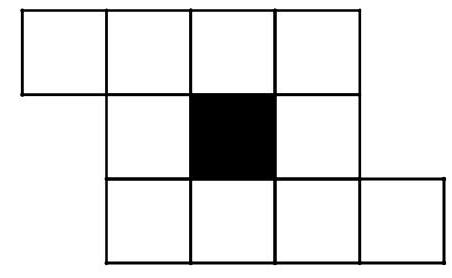
\includegraphics[max width=\textwidth, center]{2024_11_21_7e7fc96a5aa198d77b29g-1}


\end{document}